\section{Implementação}

O trabalho se iniciou em aprender como o framework Chilkat funciona criando os arquivos `spider.cpp` e `spider.h`.

Cada instância do Spider foi criado para ficar responsável por apenas um dommínio. Para evitar detecção de DDoS e tentar acessar mais páginas paralelamente.

O arquivo `main.cpp` é o que gerencia todo o processo, em que instância os \textit{spiders} e faz o escalonamento para enviar o máximo determinado de threads a cada iteração.

Para facilitar o \textit{DEBUG} (estou entregando o trabalho atrasado por causa disto xD), o escalonador é feito em cada iteração (\textit{short-term scheduler}). Quando determinado é disparado as threads responsável pra cada domínio e depois é esperado que as threads terminem para que coletem os links para criar outras threads de domínio e os guardam em arquivos temporários caso o programa pare. Como é ilustrado na figura \ref{fig1}.

\begin{figure}
  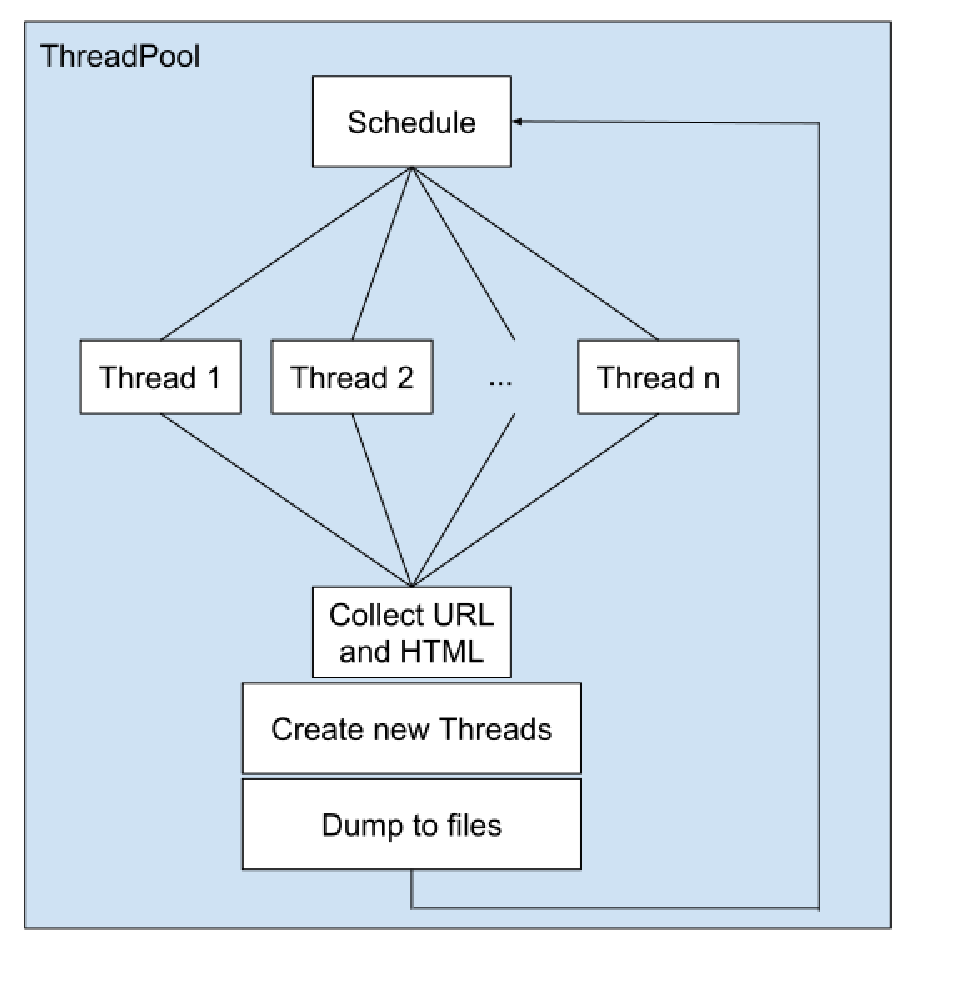
\includegraphics[width=0.6\textwidth]{images/aux1.eps}
  \caption{ThreadPool}
  \label{fig1}
\end{figure}

Portanto, um thread pode criar um gargalo, mas está setado o timeout para 10 segundos.

A fila utilizada contendo os theads para serem disparados é FIFO.

\subsection{Arquivos temporários}
Os arquivos temporários criados são:

\begin{itemize}
  \item output\_file.txt

  Arquivo contendo dump das urls e páginas html

  \item save\_state.sav

  Arquivo guarda todas as urls que estão na lista no final da iteração. Caso o programa é reiniciado, ele carrega todas as urls para que entre na fila novamente.

  \item unique\_id\_file.txt

  Coleção de hashs em \textit{unsigned long long}, calculado com \textbf{URL + HTML}, assim é detectado se uma página já foi acessada e assim ignorada. E páginas atualizadas como \textbf{g1.globo.com} são novamente acessadas.

\end{itemize}

Lembrando que o comando `make clean` deleta o conteúdo destes arquivos.
